\section{Gráficos adicionales}

Como se comentó en la sección 2, el análisis de la centralidad de los actores de la red, se han realizado algunos gráficos adicionales para poder visualizar los actores principales de la red:

\begin{itemize}
	\item Componente gigante usando el vector propio como color y el grado como tamaño de los nodos.
	\item Componente gigante usando el vector propio como color y la intermediación como tamaño de los nodos.
\end{itemize}


\newpage
\begin{figure}[H]
	\centering
	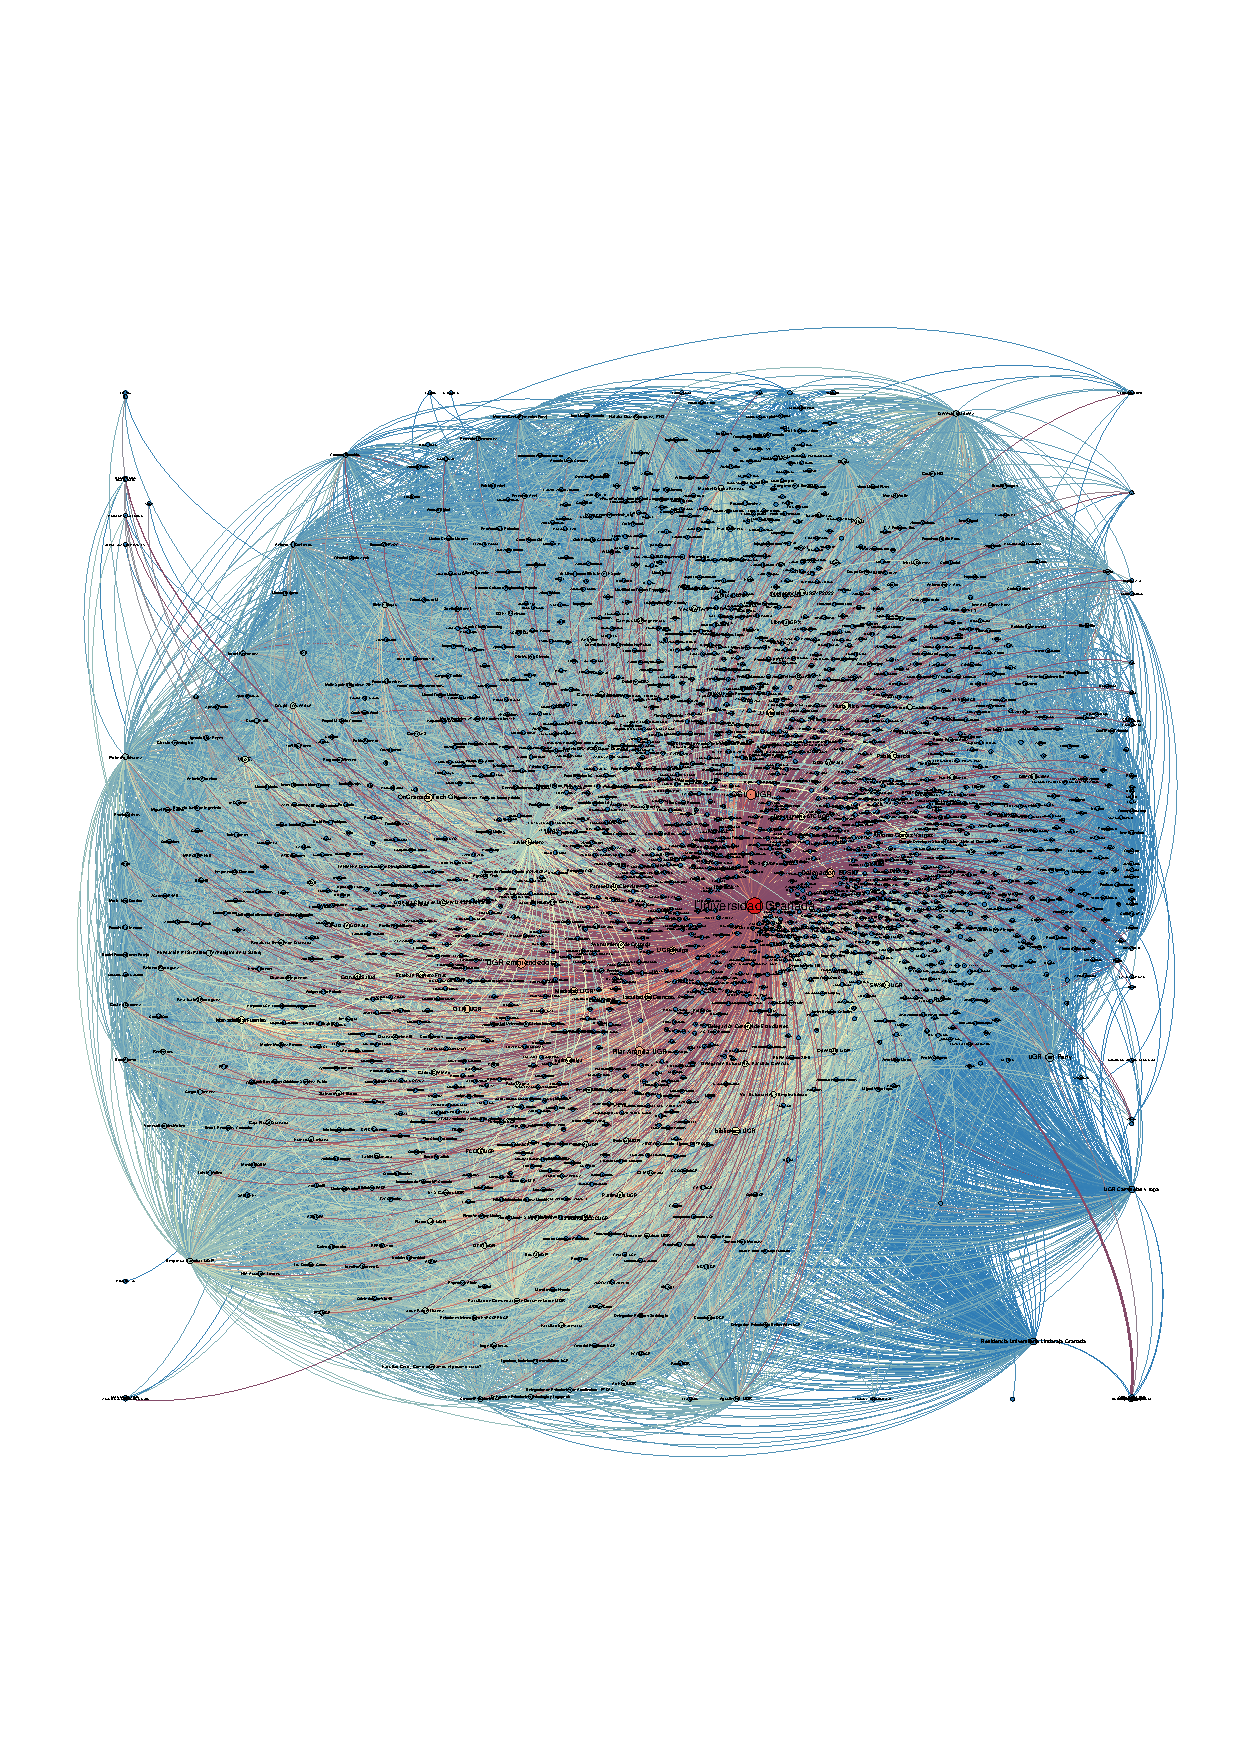
\includepdf[frame=true, scale=0.9, offset=75 -50]{pdf_incrustados/tam_grado_color_vector_propio.pdf}
	\caption{Componente gigante de la red de seguidores de la cuenta ETSIIT, coloreada según el valor de vector propio y tamaño de los nodos acorde al grado.}
\end{figure}
\vspace{18cm}
Gracias a esta visualización podemos ver que realmente la cuenta de la Universidad de Granada tiene conexiones por toda la red, al ver tantas aristas rojas por toda la red, y que los nodos que destacan son los que efectivamente hemos analizado anteriormente, la cuenta de la UGR, OSL, UGR Emprendedora y Delegación ETSIIT.
\newpage

\newpage
\begin{figure}[H]
	\centering
	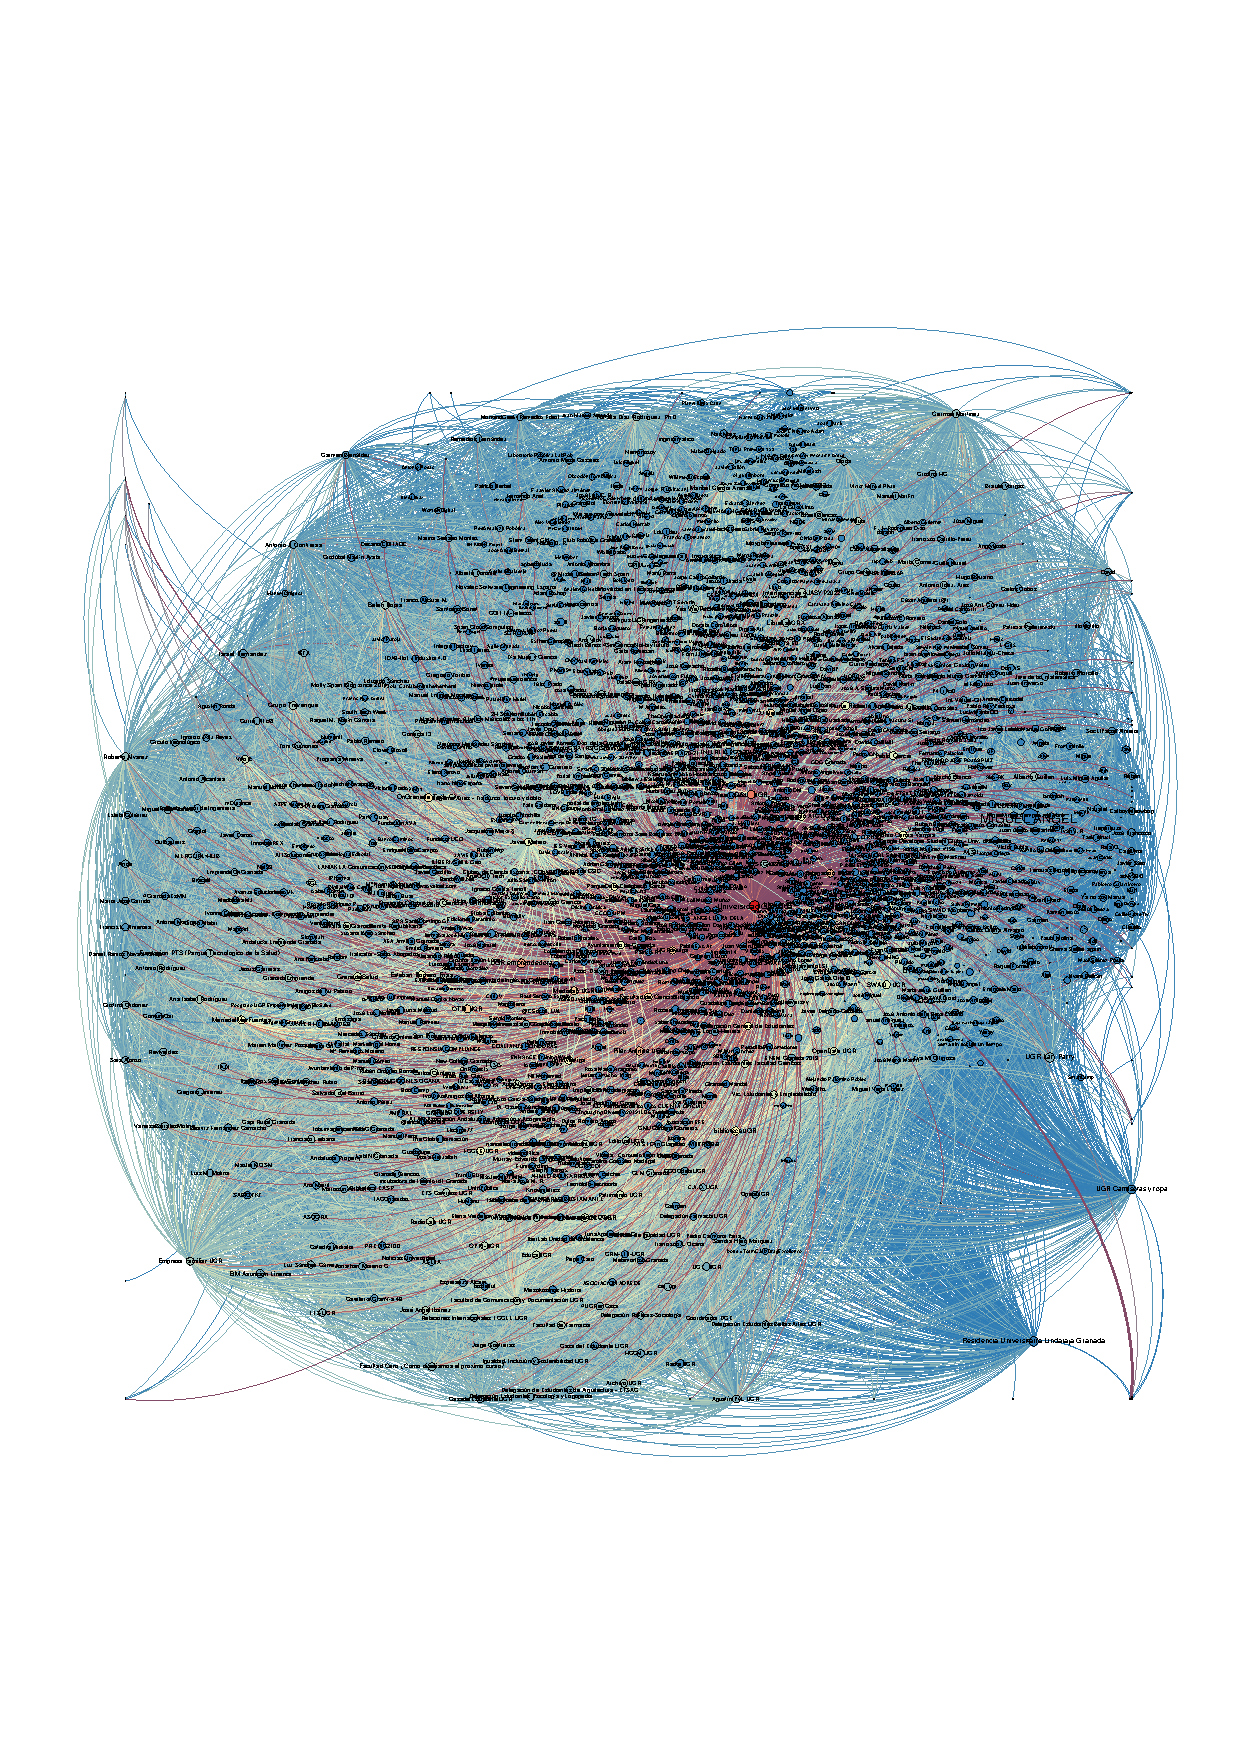
\includepdf[frame=true, scale=0.9, offset=75 -50]{pdf_incrustados/tam_intermediacion_color_vector_propio.pdf}
	\caption{Componente gigante de la red de seguidores de la cuenta ETSIIT, coloreada según el valor de vector propio y tamaño de los nodos acorde al valor de intermediación.}
\end{figure}
\vspace{18cm}
En este caso ocurre como en la visualización anterior, aunque se destaca bastante bien el caso raro que hemos encontrado en la cuenta de Miguel Ángel, al tener un tamaño de nodo muy grande, sin embargo se un color azul muy frio. Como vemos estas visualizaciones se corresponden a lo que hemos analizado en la segunda sección, pero el usar estos valores para visualizar la red nos permite hacer un mejor análisis a primera vista que cuando se presentó la red completa. 
\newpage
